\documentclass[a4paper,12pt,notitlepage]{article}
\usepackage{fullpage}
%\setkomafont{disposition}{\normalfont\bfseries}
%\usepackage{setspace}
%\setstretch{1.5}
\usepackage{graphicx}
\usepackage{tikz}
\usetikzlibrary{shapes,arrows,positioning}
\usepackage[style=authoryear,backend=biber]{biblatex}
\renewcommand*{\nameyeardelim}{\addcomma\addspace}
\usepackage[toc,page]{appendix}
\newcommand{\source}[2]{\emph{#1
} (appendix~\ref{#2}, page~\pageref{#2})}
\newcommand{\secref}[1]{(section~\ref{#1}, page~\pageref{#1})}
\usepackage{textcomp}
\usepackage{amsmath}
\usepackage{mathtools}
\usepackage{listings}
\newcommand{\code}[1]{\colorbox{white}{\lstinline[basicstyle=\ttfamily\color{black}]|#1|}
}
\usepackage{color}
\usepackage{hyperref}
\addbibresource{report.bib}
\graphicspath{{res/images/}}

\begin{document}

\parskip 2mm

\title{{\huge Playing Card Recognition}\\\vspace{2 mm}{\large \textbf{Computer Vision (EE4H) --- Final Report}}}
%\subtitle{EECE MEng4 FYP -– Second Report}
\author{Yousef Amar (1095307)\\Chris Lewis (1234567)}
\date{2014-04-28}
\maketitle
\thispagestyle{empty}
\vfill
%\begin{quotation}
\begin{abstract}
	Lorem ipsum dolor sit amet, consectetur adipisicing elit, sed do eiusmod tempor incididunt ut labore et dolore magna aliqua. Ut enim ad minim veniam, quis nostrud exercitation ullamco laboris nisi ut aliquip ex ea commodo consequat. Duis aute irure dolor in reprehenderit in voluptate velit esse cillum dolore eu fugiat nulla pariatur. Excepteur sint occaecat cupidatat non proident, sunt in culpa qui officia deserunt mollit anim id est laborum.
\end{abstract}
%\end{quotation}
\pagebreak

%\addtocontents{toc}{\protect\thispagestyle{empty}}
\tableofcontents
\thispagestyle{empty}
\pagebreak
\setcounter{page}{1}

\parskip 2mm

\section{Introduction}
	\subsection{Task Assigned}
	\subsection{Method Used}
	\subsection{Findings}
\pagebreak
\section{Review}
	\subsection{Identify sub-tasks}
		(Flowhart breakdown from final PPT?)
	\subsection{Review of methods}
		(existing literature (HIPR2?))
		Should each include limitations if not chosen, justification in 3.2
		\subsubsection{High-level Isolation}
			Contours
			Perspective transform (That OpenGL citation?)
		\subsubsection{Low-level Classification}
			Basic morphology
			HoM Transform
\pagebreak
\section{Proposed Method}
	\subsection{Logical progression from whole image to classification}
		Program flow, flowchart
	\subsection{Justify each stage’s techniques}
		Identify strengths and weaknesses
\pagebreak
\section{Implementation}
	Justify custom implementations vs. OpenCV pre-made function
	\^(interleaved and when relevant)
	\subsection{Image IO/Webcam IO}
	\subsection{Card Isolation}

		Once an image is passed in as an input, the first step is to find one or more cards in the image and, if any were found, extract them from the image and prepare them for processing. This is done in a number of steps.

		\subsubsection{Card Detection}

			In order to detect cards within the image, the function \code{find_cards()} in \source{isolation.cpp}{app:maincpp} is called from \source{main.cpp}{app:maincpp}. It takes in an empty vector of objects of type \code{Card} as an inputs which it then populates with the detected cards for later processing.

			Cards are detected by finding quadrilaterals with a method not unlike the one used in the sample file \emph{squares.cpp} in the official OpenCV repository \autocite{squares} albeit with some decisive distinctions. The backbone of the algorithm is the OpenCV function \code{cv::findContours()}. This function retrieves contours from a binary image using the algorithm developed by \textcite{suzuki1985topological} via border following. It was decided not to implement a custom function since it would not have added any flexibility or speed advantage over the OpenCV implementation. Indeed it would only have increased code complexity.

			% TODO: Label "High-level Isolation"
			This function requires a binary image as an input. As such, input images undergo a series of processing before hand. First, they are converted to greyscale. Then CLAHE --- as explained previously \secref{sec:isolation} --- is applied to these images. The size of the CLAHE window varies between 32x32 and 28x28 pixels depending on if the user has specified with the \code{--multi} command line flag that the program should run in multiple card mode. CLAHE operations using OpenCV functions run on the GPU through CUDA; they cannot be optimised by writing custom code for CLAHE without utilising CUDA, which would only introduce system-level bugs that have been long since resolved within OpenCV's code base. For this reason, the OpenCV CLAHE implementation was used.

			% TODO: IMAGES

			After performing CLAHE, the image is blurred. The amount of blur is set as a function of it image's dimensions. More specifically \code{(image_size.width + image_size.height)>>8} or in plain English, the perimeter of the image divided by 512. This prevents small images from losing too much detail through blurring while large images do not remain too sharp. Blurring is done to filter out noise for the next step.

			The resulting image is then converted to binary using the threshold parameter before \code{cv::findContours()} is called. Contours are found for processed binary images for thresholds ranging from 150 to 255 (both inclusive) in increments of 2. This bright range was experimentally determined to be the best to create binary images from.

			The found contours are then approximated into geometry using with the function \code{cv::approxPolyDP()} and then go through a number of rigorous checks. Contours that do not pass these checks are discarded and not added to the final contours collection that the function populates. These include:

			\begin{enumerate}
				\item Does the contour have four corners?\\[4px]
					Although card contours can have more than 4 approximated corners if the cards are bent or folded significantly, most will not, so the design does not handle card contours with more than four corners.
				\item Is its area greater than 4\% of the whole image?\\[4px]
					This is to filter out noise.
				\item Is it convex in shape like card borders?
				\item Is its area less than 75\% of the image?\\[4px]
					This is to filter out borders.
				% TODO: More detail? Including reason for fixing?
				\item Is it not inside another previously detected contour or another inside it?\\[4px]
					Calculated mathematically from vertex coordinate information. This is to filter out symbol (e.g. diamonds) and picture card misclassification. Previously detected contours in the list that turn out to be contained by newly detected contours are replaced by the newly detected and discarded.
				\item Is it significantly dissimilar to previously detected contours?\\[4px]
					The criteria for this check are that every rotation of the four contour vertices are at least a certain total distance away from their counterparts (summed up manhattan/city block distance in pixels). This minimum total distance is a function of the image size to normalise pixel units into units relative to the image dimensions. This relationship is \code{(image_size.width + image_size.height) * 0.5F * min_square_diff} or in other words, the mean image side length (to account for disproportionate image aspect ratios) multiplied by a constant factor set to $0.1$, i.e. 10\% of the mean image side length.
			\end{enumerate}

			Once all contours have been iterated through and the ones that fail these criteria have been filtered out, the result is a collection of contour quads that surround at least every card in the image (in the form of a \code{vector<vector<cv::Point> >} --- a vector of vectors with four points each). \emph{At least} every card in the image; the pruning process is not yet over!

			The assortment of contours go through a secondary, later filtration process that requires processing the pixel data within these contours. To do this --- as well as to construct the card Mats for subsequent classification --- the contour quad data is used to perspective transform the original image into a rectangular image of the card, an operation reviewed previously \secref{sec:isolation}.

			\begin{figure}[ht]
				\centering
				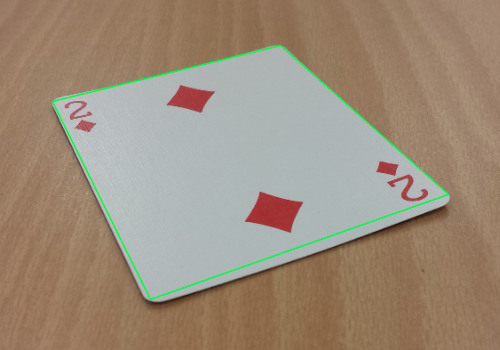
\includegraphics[width=0.6\linewidth]{perstrans1}
				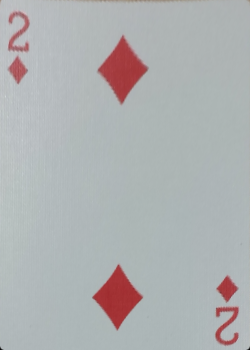
\includegraphics[width=0.3\linewidth]{perstrans2}
				\caption{Output of Perspective Transform of Contour Quad from Test Image}
				\label{fig:perstrans}
			\end{figure}

			The perspective transform is low-level enough that its implementations do not vary much at all. The maths involved in calculating the 3x3 matrix of a perspective transform that can be used to map pixels at a perspective to other shapes/perspectives is standard but cumbersome to implement (unlike an affine transform). For these reasons, the OpenCV function \code{cv::getPerspectiveTransform()} was used. It takes two quads as inputs and returns the map matrix. The source quad is the detected contour and the destination quad is a simple 250x350 rectangle which matches the standard 5:7 poker card aspect ratio like in figure~\ref{fig:perstrans}.

			The transformation matrix is then used in the function \code{cv::warpPerspective()} which deforms the pixel grid of the source image and maps it to the destination image while interpolating transitional pixels; a process that is both non-trivial as well as distant from the task at hand. The Mat produced through this process is subsequently used to instantiate a new \code{Card} object.

			On instantiation, the \code{Card} constructor additionally generates an 8x8 CLAHE version and a 140 threshold binary version of the card Mat, which are publicly accessible from a \code{Card} object. Once instantiated, the cards binary Mat is finally used for the last phase of isolation filtering.

			The last criteria for what makes a card is its whiteness measure. The measure is simple; all non-zero (i.e. white) pixels in the card Mat are counted and the final value is divided by the card's area giving a float that describes the proportion of whiteness in the card. The whiteness threshold is set to an experimentally practical \code{0.5F} or 50\% bearing in mind that error due to lighting inconsistency is a non-issue following CLAHE. Cards that are not white enough are discarded. This solves false detections such as that in figure~\ref{fig:whiteness}.

			\begin{figure}[ht]
				\centering
				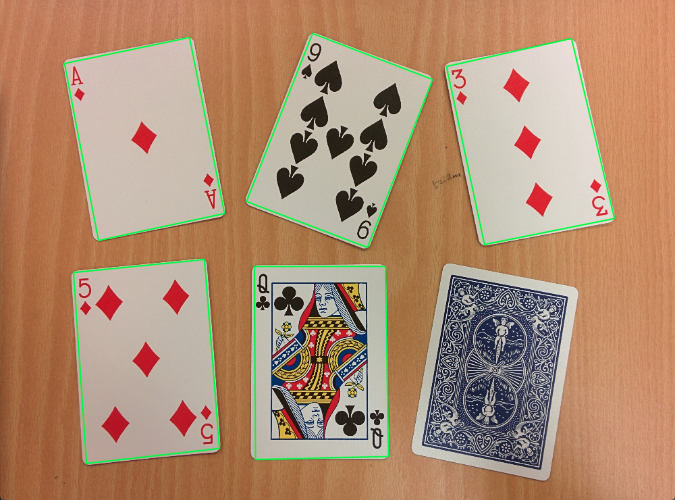
\includegraphics[width=0.9\linewidth]{whiteness}
				\caption{Example of Whiteness Check Ignoring Overturned Card}
				\label{fig:whiteness}
			\end{figure}

			Finally, there is one more processing step that needs to be undertaken before a detected card is deemed worthy enough to join its brethren in the detected card vector and \code{find_cards()} can return...

		\subsubsection{Rotation Correction}

			One deal-breaking issue was the problem of a sequence of contour quad vertices starting at the wrong corner and, as a direct consequence, causing the final card Mat to be perspective transformed incorrectly. This problem became evident became evident when processing cards where the top-most corner in the image is numbered, such as the lower examples in figure~\ref{fig:rot}; the card could just be at a very strange perspective that projects to that shape.

			\begin{figure}[ht]
				\centering
				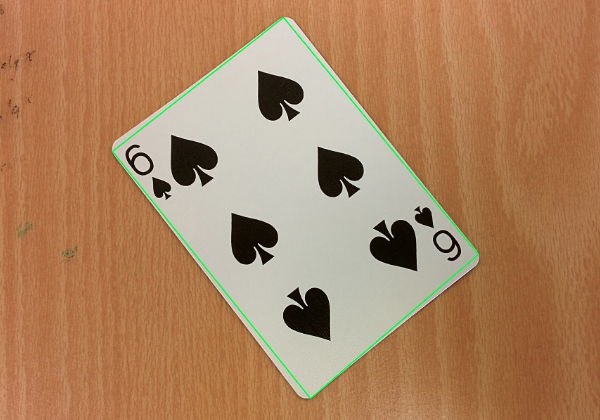
\includegraphics[width=0.6\linewidth]{rot1}
				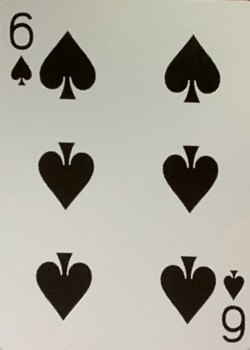
\includegraphics[width=0.3\linewidth]{rot2}\\[5px]
				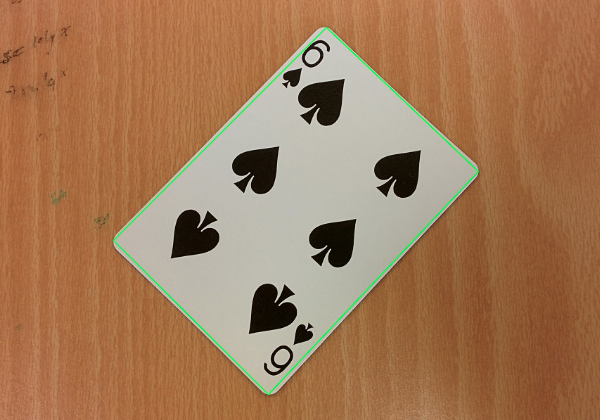
\includegraphics[width=0.6\linewidth]{rot3}
				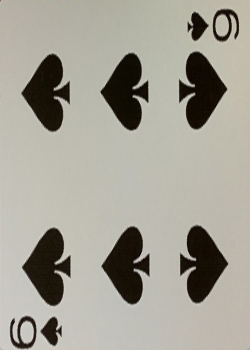
\includegraphics[width=0.3\linewidth]{rot4}
				\caption{Example of Erroneous Perspective Transformation}
				\label{fig:rot}
			\end{figure}

			The solution developed is simple and works very well. The same measure of whiteness as is used for the whole card is applied to both the top left and the bottom right corners of the card Mat (the bounds for which are defined as static constants in the \code{Card} class based on physical measurements). If corner whiteness surpasses 80\%, the card quad is rotated by one vertex --- the direction or rotation being arbitrary due to a card's symmetry --- and transformed into a new Mat.

			The corner whiteness for this new Mat is also measured, and compared against old corner whiteness. If it has a lesser corner whiteness measure than the old, that means that the old card Mat was indeed oriented incorrectly and so the new one is used instead. If the opposite holds true, then the first overall whiteness threshold was passed incorrectly (perhaps due to some bizarre specular lighting that the CLAHE did not quite catch) and so the new mat is discarded and the old one's usage is continued as if nothing ever happened.

			At long last, the \code{Card} vector contains all detected cards --- to a high degree of accuracy --- ready for processing and classification by the rest of the program, and the function can return.

	\subsection{Color Detection}
	\subsection{Type Detection}
	\subsection{Symbol/Rank symbol Isolation}
	\subsection{Number Detection}
		\subsubsection{Value cards}
			Morphological opening/closing
			Floodfill count
		\subsubsection{Picture cards}
			Application of HoM
		\subsubsection{Custom HoM Implementation}
	\subsection{Suit Symbol Detection}
		Colour Integration
		HoM
	\subsection{Results output}
		GUI
		Console output
\pagebreak
\section{Evaluation}
	\subsection{Test images, increasing complexity}
	\subsection{Webcam tests}
	\subsection{Confusion Matrix}
\pagebreak
\section{Conclusion}
	\subsection{Summary}
	\subsection{Improvements}
\pagebreak
\begin{appendices}
	\section{Contribution Agreement}
		(I have both of these and can scan them)
	\pagebreak
	\section{Source Code Listings}
		\definecolor{bluekeywords}{rgb}{0.13,0.13,1}
		\definecolor{greencomments}{rgb}{0,0.5,0}
		\definecolor{redstrings}{rgb}{0.9,0.7,1}

		% Here's where you can mess with the style (this is a comment btw)
		\lstset{
			language=C++,
			showspaces=false,
			showtabs=false,
			breaklines=true,
			breakatwhitespace=true,
			escapeinside={(*@}{@*)},
			commentstyle=\color{greencomments},
			keywordstyle=\color{bluekeywords},
			stringstyle=\color{redstrings},
			basicstyle=\ttfamily\scriptsize,
			captionpos=t,
			extendedchars=true,
			frame=single,
			keepspaces=true,
			showstringspaces=false,
			stepnumber=2,
			tabsize=2,
		}

		\subsection{main.cpp}
		\label{app:maincpp}
		\lstinputlisting{res/appendices/src/main.cpp}
\end{appendices}

\vfill
\hrulefill

\end{document}

\section{Introduction}
	
	This is a paragraph. Here's an example of cross-referencing: please see Review (section \ref{sec:review} on page \pageref{sec:review}).

	\subsection{Project Specification}

		This is a \emph{subsection}. Whitespace is mostly meaningless in \LaTeX. Indenting with tabs is just useful for collapsing parts of the document you aren't working on in Sublime; it has no effect on document appearance. Speaking of Sublime, these are some useful packages for working in \LaTeX:

		\begin{enumerate}
			\item ``LaTeXTools'' (better than ``LaTeXing'') because
			\begin{enumerate}
				\item Doesn't pester you to buy it
				\item Has pretty good syntax highlighting and auto completion
				\item Auto completion for cross-referencing figures/sections/appendices and citations too
				\item Includes LaTeX build system --- Ctrl+B to compile; no command line headaches
			\end{enumerate}
			\item Edit your settings file for really smooth spell check: \url{http://www.sublimetext.com/docs/3/spell_checking.html}
			\item ``Origami'' for multiple panes in Sublime --- useful to have notes open as a clipboard on the side
			\item ``Increment Selection'' (came in handy once or twice)
		\end{enumerate}

\pagebreak

\section{Review}
\label{sec:review}

	Here's another section. Here's a figure with 0.8 of the line width:

	\begin{figure}[ht]
		\centering
		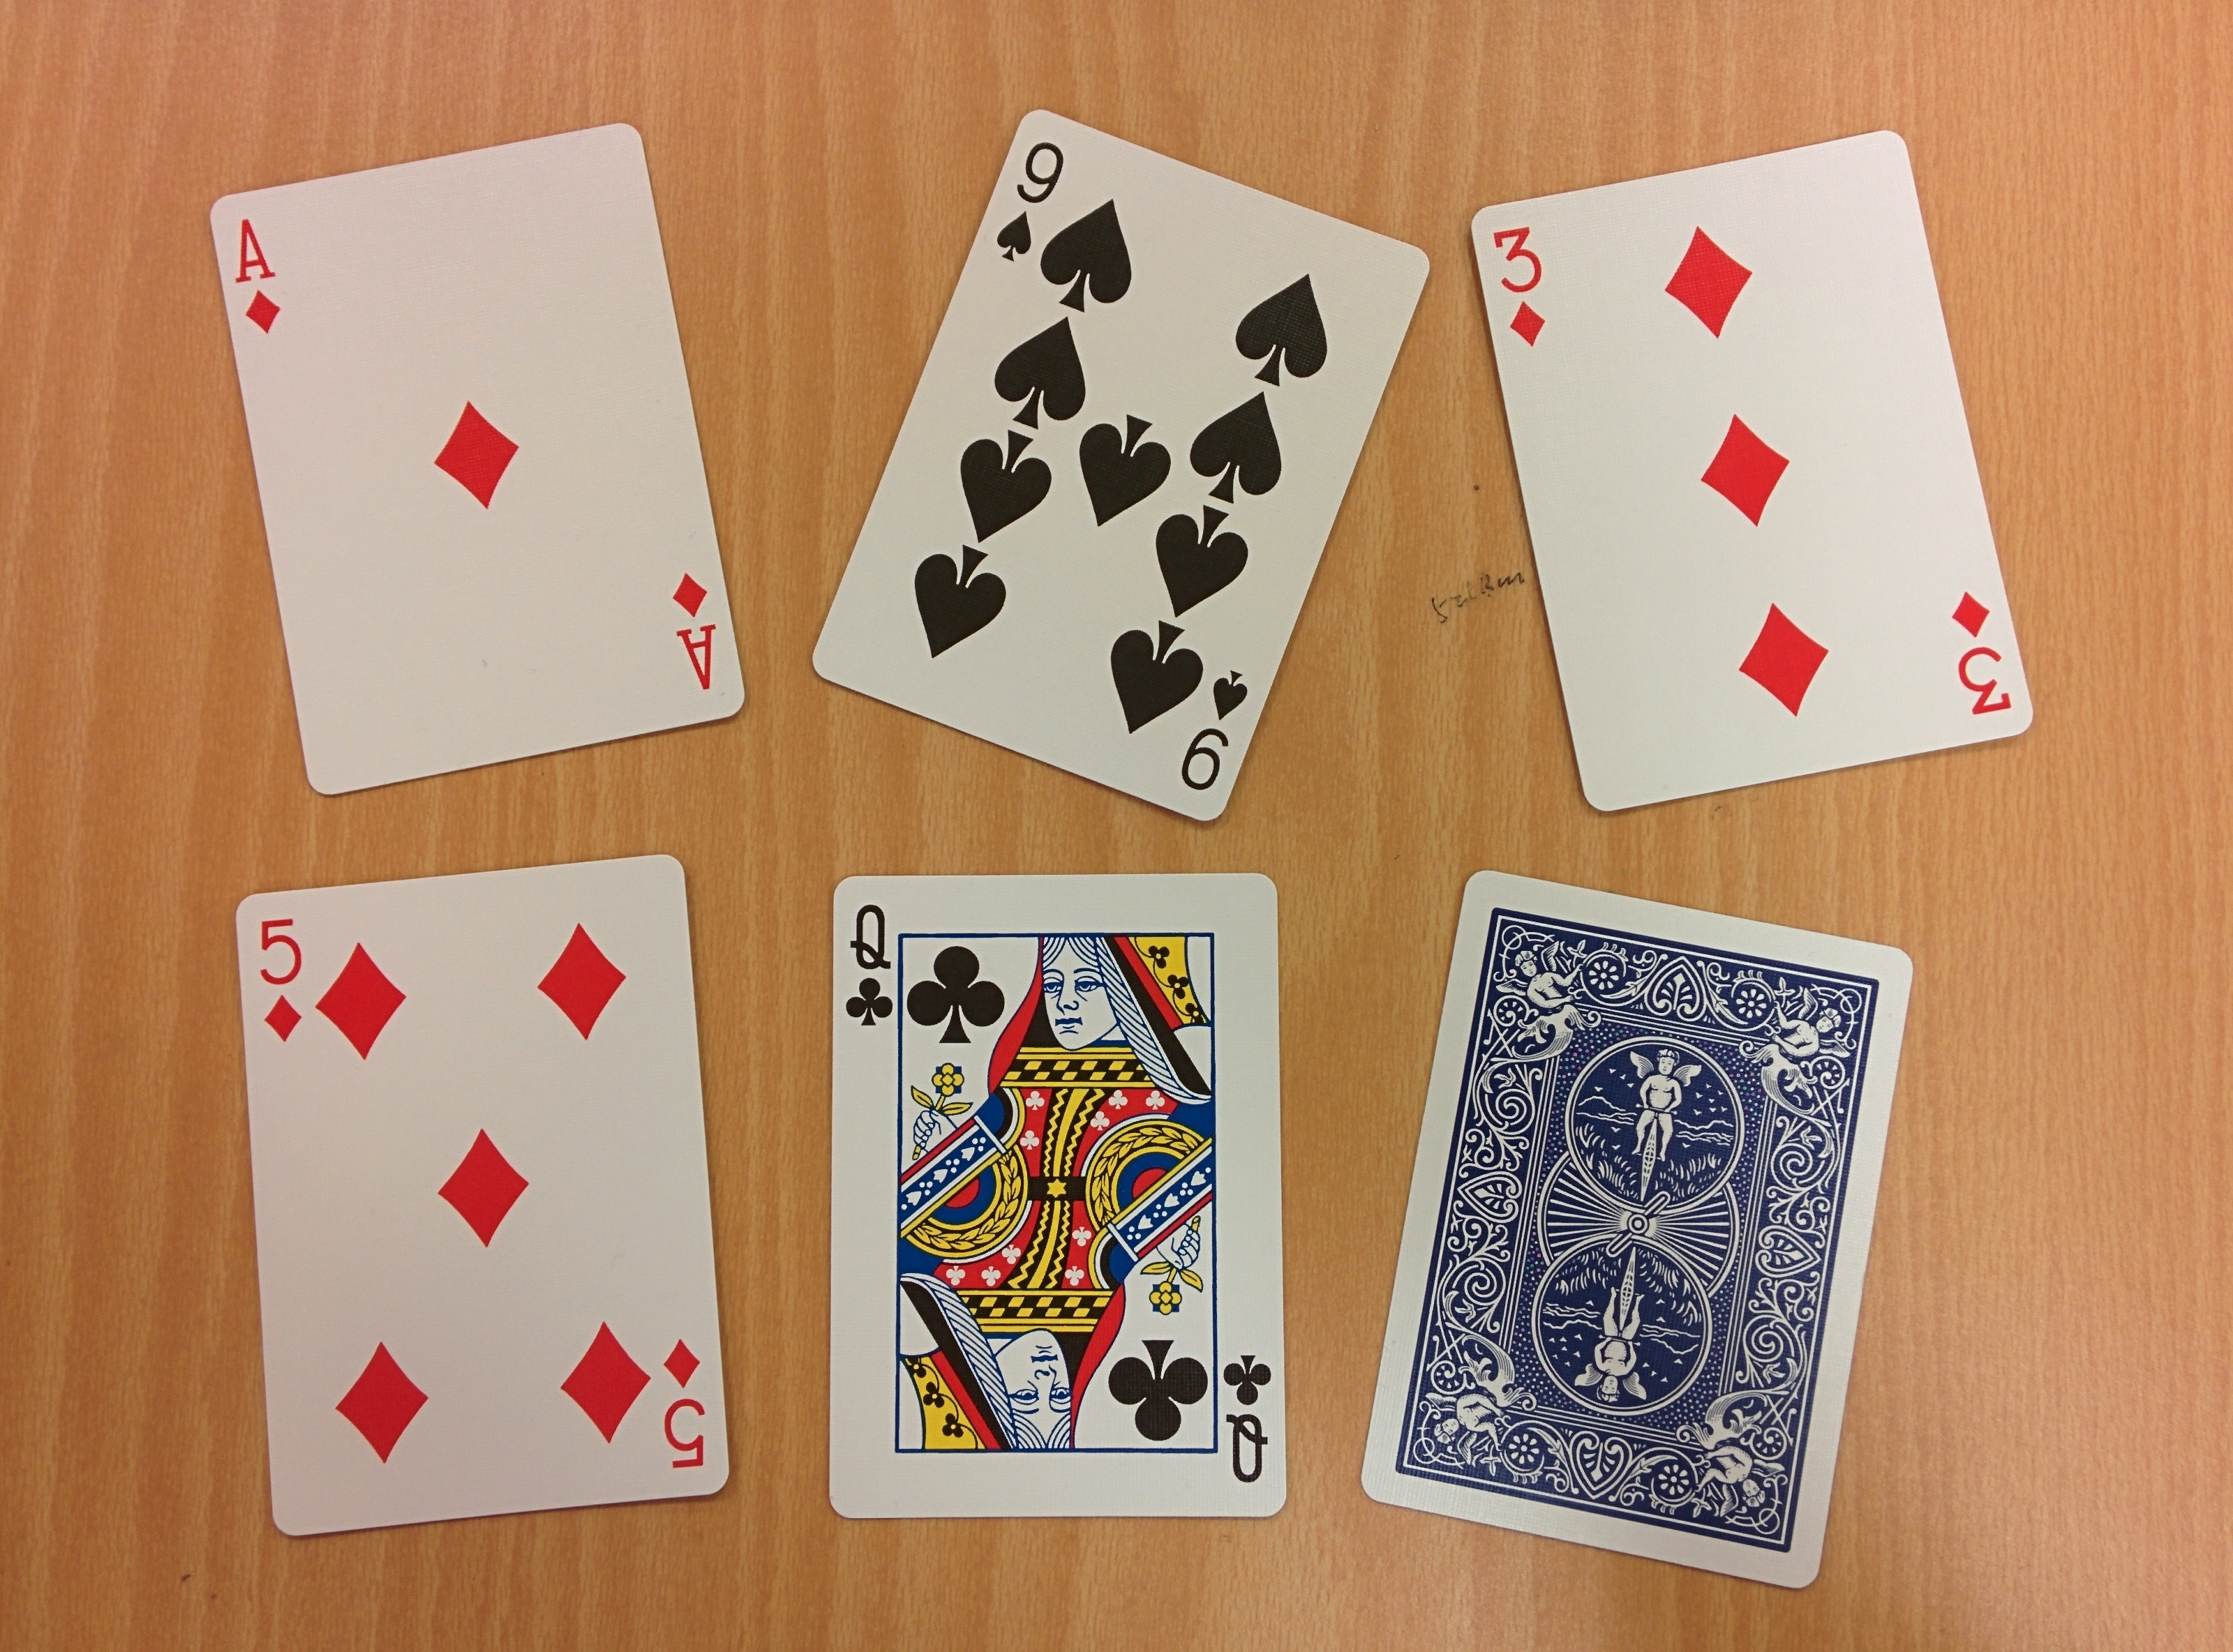
\includegraphics[width=0.8\linewidth]{mixed}
		\caption{Example of Card}
		\label{fig:mixed}
	\end{figure}

	\LaTeX is pretty good at figuring out what to do with figure. There are a number of options for them too that are cool. Here's me cross-referencing the figure without breaking a sweat: please see figure \ref{fig:mixed} on page \pageref{fig:mixed}.

\pagebreak

\section{Proposed Method}

	\LaTeX is really good at equations. Here's a simple one from my report:

	$$x = \frac{ct}{2} - \epsilon$$

	Want some confusion matrices? Here are some matrix examples from my final report:

	\begin{equation*}
		T =
		\begin{bmatrix}
			84 & 200 & 16 \\
			56 & 238 & 11 \\
			251 & 206 & 203
		\end{bmatrix}
		\qquad
		I =
		\begin{bmatrix}
			160 & 40 & 250 & 27 & 114 \\
			81 & 94 & 14 & 100 & 37 \\
			225 & 52 & 148 & 137 & 111
		\end{bmatrix}
	\end{equation*}

	Here's me sprinkling some math inline: $\theta$, $x$ and $y$, $I_1$ and $I_2$, $|T - I_n|$. Want some graphs? Google pgfplots and prepare to be blown away.

\pagebreak

\section{Implementation}
	
	You can also put a lot of stuff in one figure even on different lines:
	
	\begin{figure}[ht]
		\centering
		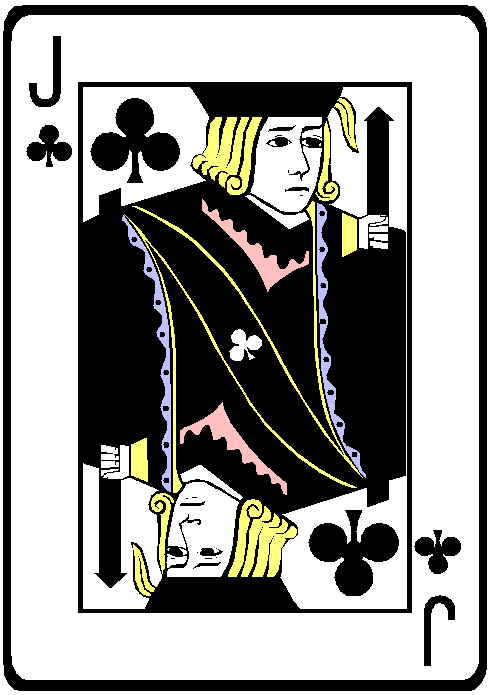
\includegraphics[width=0.2\linewidth]{cards/jackofclubs}
		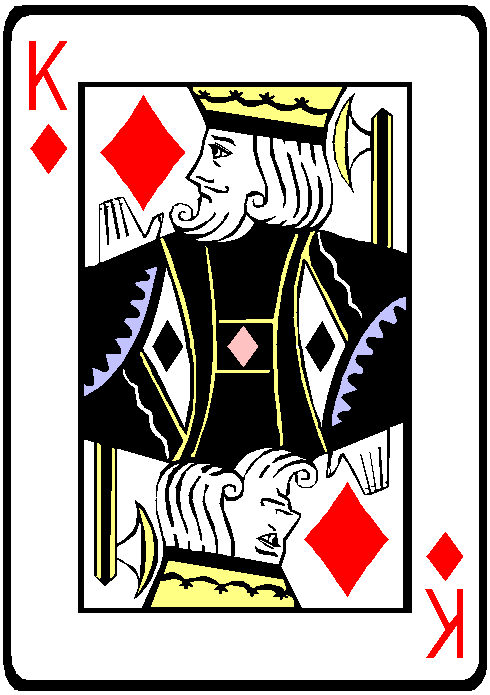
\includegraphics[width=0.2\linewidth]{cards/kingofdiamonds}
		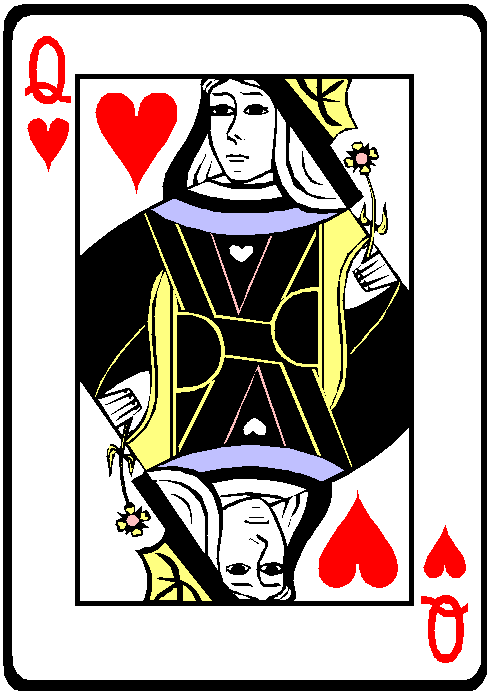
\includegraphics[width=0.2\linewidth]{cards/queenofhearts}\\[5px]
		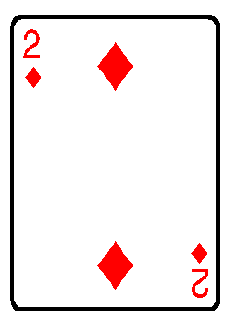
\includegraphics[width=0.3\linewidth]{cards/2ofdiamonds}
		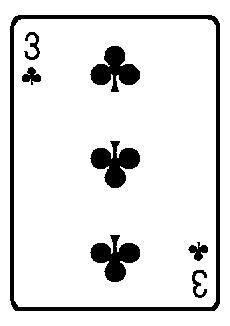
\includegraphics[width=0.3\linewidth]{cards/3ofclubs}
		\caption{Example of Cards}
		\label{fig:stuff}
	\end{figure}

\pagebreak

\section{Evaluation}
	
	See appendix \ref{app:maincpp} on page \pageref{app:maincpp} for an example of code listings. The style is completely customisable of course. Notice also that it's not copied to the \emph{appendices} directory, it's just a symlink to \emph{src}! According to this random book off of Google Scholar, computer vision is pretty cool \autocite{forsyth2002computer}. I use BibLatex + Biber to compile the bibliography; the order is ``latexmk'' (or build), ``biber report'', then ``latexmk'' again. This only needs to be done if the bibliography changes and then it might as well be done only really at the very end when the report is finished to so don't worry about it. LaTeXing does it automatically but it's not worth it.

\pagebreak

\section{Conclusion}

	We've only just scratched the surface! Here, have a mini flow chart:

	% Define block styles
	\tikzstyle{decision} = [diamond, draw, fill=blue!20, text badly centered, inner sep=0pt, text width=4em, font=\tiny]
	\tikzstyle{process} = [rectangle, draw, fill=blue!20, text centered, rounded corners, text width=3em, font=\tiny]
	\tikzstyle{line} = [draw, -latex', font=\tiny]
	\tikzstyle{cloud} = [draw, ellipse, fill=red!20, minimum height=2em]
	
	\begin{figure}[ht]
		\centering
		\begin{tikzpicture}[node distance = 2cm, auto]
			% Place nodes
			\node [process] (imgget) {Get Image from File/Webcam};
			\node [process, right of=imgget] (cardfind) {Isolate Cards};
			\node [process, right of=cardfind] (colourdet) {Detect Colour};
			\node [process, right of=colourdet] (typedet) {Detect Type};
			\node [process, right of=typedet] (symfind) {Isolate Symbols};
			\node [decision, right of=symfind] (ispic) {Is Card Picture Type?};
			\node [process, above right of=ispic] (numdet) {Detect Number};
			\node [process, below right of=ispic] (rankdet) {Detect Rank};
			% Enhanced by colour detection
			\node [process, below right of=numdet] (symdet) {Detect Suit};


			% Draw edges
			\path [line] (imgget) -- (cardfind);
			\path [line] (cardfind) -- (colourdet);
			\path [line] (colourdet) -- (typedet);
			\path [line] (typedet) -- (symfind);
			\path [line] (symfind) -- (ispic);
			\path [line] (ispic) -- node {no} (numdet);
			\path [line] (ispic) -- node [below left] {yes} (rankdet);
			\path [line] (rankdet) -- (symdet);
			\path [line] (numdet) -- (symdet);
			%\path [line,dashed] (expert) -- (init);
			%\path [line,dashed] (system) -- (init);
			%\path [line,dashed] (system) |- (evaluate);
		\end{tikzpicture}
		\caption{Top-level Flowchart}
		\label{fig:flowchart}
	\end{figure}

\pagebreak

\thispagestyle{empty}
\printbibliography


\end{document}